\newpage
\chapter{Prediction Heuristics}
\label{chapter02}

Heuristic algorithms are an approach to solving computational problems based on experience and intuition. This algorithm does not guarantee an optimal solution for the given task. Heuristic algorithms are widely used in tasks that are difficult to amenable to exact numerical methods or analytical solutions. Although they cannot offer an optimal solution, heuristic algorithms\index{heuristic algorithms} often lead to sufficiently acceptable in practice close to optimal solutions. Due to their non-deterministic nature, heuristic algorithms\index{heuristic algorithms} are highly suitable for implementation in supercomputer computing\index{supercomputer computing}. Two extremely popular heuristics\index{heuristics} are artificial neural networks\index{artificial neural networks} and genetic algorithms\index{genetic algorithms}. They have been trendy in the last two decades, which gives reason to include them in the main presentation of this teaching aid. By themselves, heuristics are useless unless they are applied to a sufficiently complex computational task. This is precisely the kind of complexity that forecasting tasks offer. Forecasting is embedded in many activities of daily human life, starting with average daily temperatures and reaching the consumption of specific goods and services. In one form or another, almost every human activity is valued in terms of financial resources. This fact gives reason to examine precisely forecasts of the change in the prices of various financial instruments. Reporting the difference in price at specific intervals (equal or unequal) leads to the presentation of the information in a time series\index{time series}. In the case of time series\index{time series}, the abscissa axis indicates the time, and the ordinate axis indicates the value of the measured quantity (in this case, the price).

\section{Artificial Neural Networks}

Artificial neural networks\index{artificial neural networks} have emerged due to attempts to build a mathematical model for biological nervous systems. These systems learn (progressively improve their capabilities) by examining sample data. Their application is mainly in tasks for which traditional algorithms do not give acceptable results. Artificial neural networks are most widely used in classification tasks. According to the information in the past periods, the artificial neural network\index{artificial neural networks} can divide the data into two main classes - data showing an upward change or data leading to a downward shift. Regarding financial time series, two events are possible - an increase in value or a decrease in value.

\begin{figure}[h]
\centering
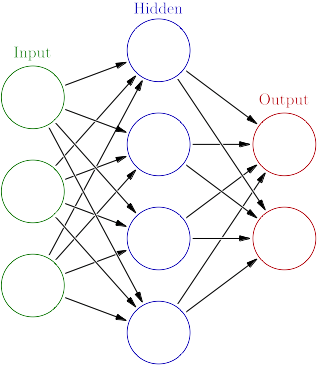
\includegraphics[height=0.25\pdfpageheight]{pic0004}
\caption{Three Layer Artificial Neural Network}
\label{fig:pic0004}
\end{figure}

The structure of classical artificial neural networks\index{artificial neural networks} consists of nodes called artificial neurons and connections called weights (Fig. \ref{fig:pic0004}). Connections between neurons serve to transmit a signal from one neuron to another. Neurons that receive signals process them according to a predetermined rule and can then, in turn, propagate them to other neurons. In the classic case, neurons have a value (usually a real number). A value also represents the connections between neurons, and according to the learning rule, precisely this value is subject to change so that the network learns the necessary information. In the most used artificial neural networks\index{artificial neural networks}, neurons are organized into layers. Signals in this type of network propagate from the input layer to the output layer, bypassing the intermediate layers. This propagation of signals is called pass in the right direction and is characteristic of the mode of use. Besides the use mode, artificial neural networks\index{artificial neural networks} also operate in a second mode called training mode. Over the past few decades, many ways to train artificial neural networks have been proposed, with the most significant results obtained using the backpropagation algorithm\index{backpropagation}. Error backpropagation is an accurate numerical method from the family of gradient methods that relies on the error that the network makes when executing the training examples. This error is detected in the output layer and propagated back through the previous layers, hence the method's name.

Due to its linear nature, backpropagation of the error\index{backpropagation of the error} is challenging to implement in parallel programming. If we look at the weights in an artificial neural network as a multidimensional infinite space of real numbers, then finding values for the weights is a mathematical optimization problem. Exact numerical methods give good results in small spaces but encounter severe difficulties in larger dimensions. Precisely opposite to exact numerical methods, heuristic algorithms provide acceptable solutions in a reasonable time. The advantage is not only efficiency but also significantly more opportunities to implement heuristic algorithms in parallel programming.

Classical neurons implement a transfer function and an activation function. The most commonly used transfer function is the linear one, which is a sum of multiplying the input signals by the weights that deliver them. The most widely used activation functions are the sigmoid function (\ref{equation02}) and the hyperbolic tangent (\ref{equation03}).

\begin{equation}
\label{equation02}
z_{j} = \frac{1}{1 + e^{-y_{j}}}
\end{equation}

\begin{equation}
\label{equation03}
z_{j} = \frac{e^{2y_{j}}-1}{e^{2y_{j}}+1}
\end{equation}

The activation function has a significant role in normalizing the output signal. This normalization is necessary because different numbers of signals are input to the transfer function at different neurons, and without normalization, this would make the output signals incommensurable. In gradient exact numerical methods, there is a requirement that the activation function is differentiable, which is unnecessary for heuristic algorithms.

\begin{equation}
\label{equation01}
y_{j} = \sum_{i=1}^{} x_{i}*w_{ij}
\end{equation}

The commonly used linear transfer function (\ref{equation01}) needs to use an additional collectible called "bias". From a formal point of view, an offset can be interpreted as a weight connecting a neuron to another neuron that emits a single signal. In practice, for each layer, it is accepted to allocate a neuron emitting a single signal. Only in the output layer is it meaningless to have such a neuron since it receives no input signals, and emitting a constant unit at the output does not carry meaningful information about the functioning of the network.

From a mathematical point of view, classical neural networks can be represented by a vector (the values of the neurons) and a matrix (the values of the weights between the neurons). In this case, the propagation of signals from the input to the output would be multiplication of a vector by a number. In this tutorial, a classical three-layer network will be fed the scaled values from the past time periods, and the output will expect a predicted value for future time intervals. This concept is slightly more complex than a simple promotion/relegation qualification, but it is significantly more informative because it is expected to provide insight into a longer time frame in the future. After successfully predicting in which direction the price will change, the question of how long this fall/rise will last becomes essential.

\section{Genetic Algorithms}

Genetic algorithms are a subset of the classes of population algorithms and evolutionary algorithms. Genetic algorithms are global optimization heuristics\index{global optimization heuristics} inspired by the ideas of biological evolution. Genetic algorithms\index{genetic algorithms} find their main application in problems with a large dimensional solution space. In such issues, classical exact numerical methods often cannot offer a solution in an acceptable time. The solution to the relevant problem must be represented as a chromosome (individual) in a general population of solutions to implement a genetic algorithm. Then, by applying the basic operations of selection\index{selection in a genetic algorithm}, crossover\index{crossover in a genetic algorithm} and mutation\index{mutation in a genetic algorithm} (Fig. \ref{fig:pic0005}), individuals (solutions) should be improved.

\begin{figure}[h]
\centering
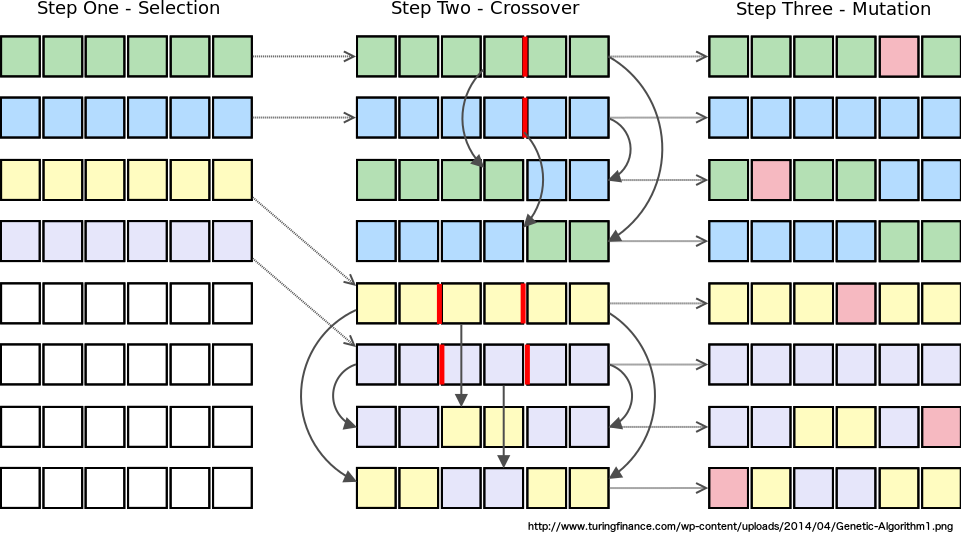
\includegraphics[width=1.0\linewidth]{pic0005}
\caption{The three basic operations in genetic algorithms}
\label{fig:pic0005}
\end{figure}

In the classical process, optimization starts from randomly generated individuals. This is optional, especially when dealing with hybrid implementations where the genetic algorithm is a supporting optimization. The initial population may be obtained in such situations due to another optimization or human arrangement. After the initial phase, the optimization proceeds iteratively and terminates according to predefined termination criteria. Most often, a predefined number of generations or the number of generations that do not lead to an improvement in the solutions found are used, but it is also possible to define an astronomical time interval.

Of fundamental importance for the successful work with genetic algorithms\index{genetic algorithms} is the determination of an objective function (life function\index{life function} of the individual), which unambiguously determines the quality of the obtained solution. Based on the different vitality that the individuals in the population have, a stochastic decision is made about which individuals will participate in the creation of the future generation and which will not. In many implementations of genetic algorithms, an elite rule is applied so that the best-discovered solution reaches the end of the optimization process. At the same time, elite rule risks degenerating the population so that all decisions favor the preserved elite.

The fact that genetic algorithms are organized based on a population of individuals suggests the ideal opportunity to manage the optimization process not in one global population but in many different local populations that exist on other computing machines. This, in turn, would enable the implementation of migration processes, just as observed in natural biological species.

\section{Financial Time Series}

Time series\index{time series} is a series of measurements performed in sequential order over time. Time series can be composed of equally spaced values or randomly spaced values. In practice, a sequence of discrete values is obtained. Often in practice, it happens that there are missing measurements, which leads to certain complications in the analysis. Financial time series generally use equal reporting intervals and rarely have missing values in reporting. Each reporting in the financial time series is distinguished by a group of values characterizing the time interval to which it refers, namely the initial value for the interval, the highest value achieved for the interval, the lowest value achieved for the interval, and the end value for the interval.

\begin{figure}[h]
\centering
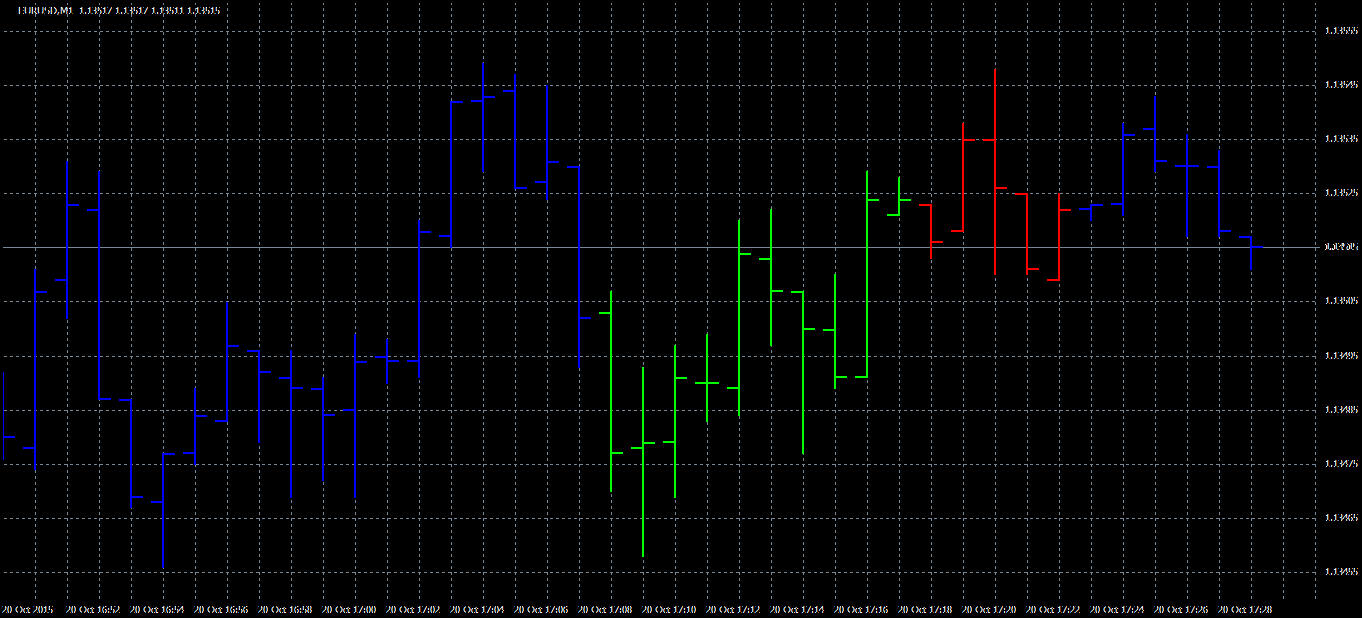
\includegraphics[width=1.0\linewidth]{pic0003}
\caption{The euro/dollar ratio within one hour}
\label{fig:pic0003}
\end{figure}

In Fig. \ref{fig:pic0003}, this information is indicated by vertical bars, with the lower end of the vertical bar symbolizing the lowest level, the upper end the highest level, and the two sidebars marking the open level (left) and the close level ( from the right). Analyzing time series\index{time series} can provide essential information for decision-makers. When it comes to time series in the financial field, the primary purpose of the analysis is to offer a forecast. One of the most commonly used forms of analysis is curve fitting. From a mathematical point of view, the task is to construct a curve that passes as close as possible to predetermined points. It is well known from mathematics that an infinite number of passing curves can be built through a finite number of points. For the fit to be meaningful, the curve must have specific properties such as smoothness, good interpolation, and extrapolation.

The conditional division of the financial time series\index{financial time series} into two halves (past and future) gives an excellent opportunity to represent the forecasting task in terms of artificial neural networks\index{artificial neural networks}. The scaled information of the past period (green in the graph) is fed to the input layer of the artificial neural network, and the forecast is obtained in the output layer of the artificial neural network and subjected to inverse scaling (red in the graph). Thus decomposed time series\index{time series} is used in the training phase of the artificial neural network. For the operational phase of the artificial neural network prediction network, the last measured values are fed without being precise about future measurements.

\section{Forecasting in a distributed environment}

The flexible ability of artificial neural networks\index{artificial neural networks} to build functional dependence between input and output data makes them an ideal candidate for a predictive system. If it is assumed that the measured values in the time series are points in a two-dimensional space, then the forecasting task can be presented as a task of passing a curve through N points (curve fitting). If the artificial neural network is figuratively likened to a polynomial, then its weights would represent coefficients in the polynomial. The values that the artificial neural network\index{artificial neural networks} generates at its output for future moments are a kind of extrapolation\index{extrapolation} according to the approximated curve. Since classical multilayer neural networks operate with input signals between 0.0 and 1.0 or -1.0 and +1.0, the time series information must be scaled to the corresponding operating interval of the network. The values of the time series are conditionally divided into past (green Fig. \ref{fig:pic0003}) and future (red Fig. \ref{fig:pic0003}). The output (predictive) information of the artificial neural network is then scaled back to the original intervals of the time series.

\begin{figure}[h]
\centering
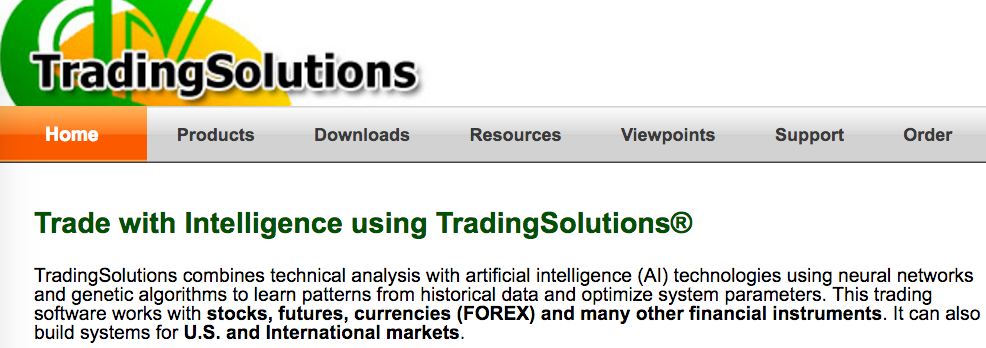
\includegraphics[width=1.0\linewidth]{pic0006}
\caption{TradingSolutions Product Line Using Artificial Neural Networks and Genetic Algorithms to Predict Forex Financial Instruments}
\label{fig:pic0006}
\end{figure}

From a purely practical point of view, using artificial neural networks and genetic algorithms has proven to be a suitable approach for forecasting financial instruments, which is visible in the TradingSolutions product line (Fig. \ref{fig:pic0006}). For almost fifteen years, the TradingSolutions product line has supplied decision support systems\index{decision support systems}. Currently, this product line has been acquired by nDimensional, Inc.

\begin{figure}[h]
\centering
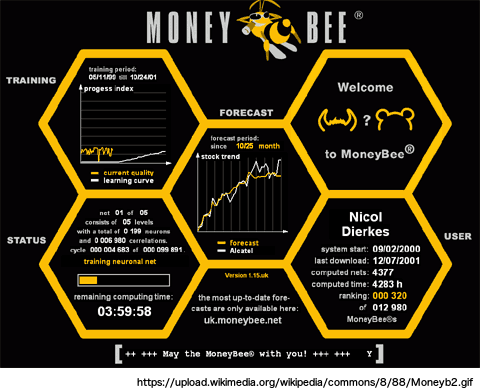
\includegraphics[height=0.4\pdfpageheight]{pic0007}
\caption{The MoneyBee system for financial forecasting in a distributed environment}
\label{fig:pic0007}
\end{figure}

The ability to predict the prices of financial instruments has always attracted industry and academic circles. One of the most notable achievements in this direction is the MoneyBee project (Fig. \ref{fig:pic0007}). Although no longer in existence, this project offered the ability to compute predictions using donated computing power\index{donated computing resources} in a distributed environment\index{distributed computing} \cite{bohn}. The actual predictions were calculated, using artificial neural networks, on users' computers during periods when the machines' load was low, and the screensaver was activated. Before the mass adoption of mobile devices, a common practice in distributed computing projects for donated computing power\index{distributed computing}, the primary approach was to perform the computations in a purpose-built monitor shielding program. After the introduction of cathode ray tubes in desktop computers, there is an effect of damage to the monitor if a static image is displayed on it for a long time. The best way to solve this problem is to have the operating system detect a period when the user is not using the computer and activate a software program to protect the monitor. The development of liquid crystal monitors gradually put cathode ray tube monitors out of use, and the use of monitor protection programs lost its original purpose. Nevertheless, this kind of software solution remains in use and mainly serves to increase information security, not only to give an aesthetic visualization but also to bring the user's work session into a locked state, which prevents the use of the computer system by unauthorized users. The availability of computing resources that are inefficiently used has led many scientists to develop remote computing systems in a distributed environment\index{distributed computing} precisely in the form of monitor protection programs that take advantage of donated user computing resources.

\section{Background calculations on mobile devices}

There is a conceptual difference in how users use their desktop computers and mobile devices. First, the desktop computer is started and stopped according to the user's needs, while mobile devices are often in continuous use mode. This leads to the main difference: mobile devices do not fall into a low-use mode but also have high-priority use modes (for example, a high-priority phone call). The second fundamental difference is that the main idea for saving electrical energy, supplied mainly by mobile device batteries, is the screen's dynamic dimming. This power-saving strategy fundamentally overturns the concept of a monitor-protecting program. To effectively implement a distributed computing system on mobile devices, it is much better to use active wallpaper technology than to rely on the idea of a program that protects the monitor. It is precisely this idea that is developed in this teaching aid.
